\subsection{Implementation}
% 
In the the prototype, we use the architecture described in Figure \ref{fig:arch-ver2-tech} as the basics for our system design. In this section //TO BE WRITTEN: SECTION OVERVIEW

The idea of the project -- to exchange cryptocurrencies -- is too broad to be implemented without further refinements. To be able to implement the prototype, we need to break this idea down to a list of desired functions or functional requirements. 

In a usual software development process, functional requirements would come from the users of the system, product owner and other stakeholders. In this project, we list the requirements for the prototype, so that the idea can be demonstrated clearly. Requirements necessary for demonstrating the idea were prioritised, the others were not worked upon. We ranked the requirements by their importance and then sorted them in a MoSCoW table. We used this table to prioritise the areas for implementation. In a market-ready product, many requirements would most likely be different.

In the previous examples, we have always considered that the two trading parties -- Alice and Bob agreed on the terms of the transaction beforehand using a separate channel. For this prototype, we have decided to include a communication channel, to enable users interact and agree on the transaction terms within the prototype. While this functionality is certainly not novel, nor it is the focus of this project, it complements the prototype and showcases, how it could be used in real-world.

\subsubsection{System components}
The prototype is implemented as an Android application. It communicates with Ethereum blockchain via Ethereum node, to deploy a custom smart contract, which operates logic described in figure \ref{fig:simple-logic} on page \pageref{fig:simple-logic} and with a back-end that facilitates the communication channel. To operate its logic, the smart contract communicates with an oracle. The oracle queries a blockchain explorer provider to learn about the status of a transaction and sends the updates back to the smart contract. User triggers the events in the Android application and validates events on the blockchain. The validation should be done with use of other systems than the Android application itself. Figure \ref{fig:system-overview} depicts the system parts and their relations. The over-all goal is to avoid a single point of failure by avoiding centralisation of `business critical' tasks\footnotemark. The following sections describe, how different parts of the system help to achieve this.
% 
\footnotetext{By \textit{business critical} is meant the process of deploying a contract and carrying out a transaction. Maintaining a communication channel for the users is \textit{not} business critical, because users may decide to rather use another existing communication channel at any time.}
% 
\begin{figure}[p]
    \centering
    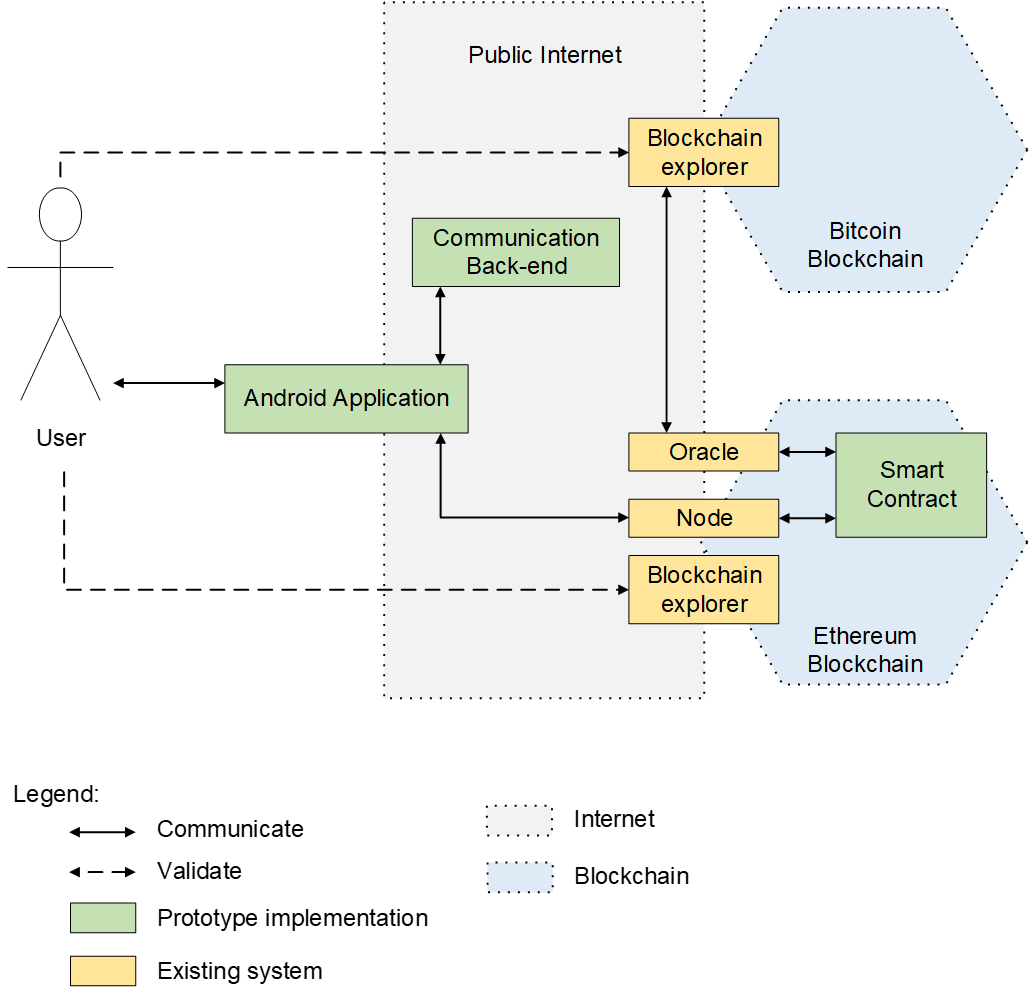
\includegraphics[width=\textwidth]{system-overview}
    \caption[itemize]{
    Overview of the system parts:
    \begin{enumerate*}[label=(\roman*)]
        \item \textit{User} communicates directly with the Android application and verifies data on the blockchain.
        \item \textit{Android application} fetches data about existing offers from the communication back-end and sends new smart contracts to the Ethereum node.
        \item \textit{Node} communicates with other nodes in the Ethereum network, maintains the status of the blockchain and deploys new smart contracts to the network.
        \item \textit{Smart contract} contacts oracle after deployment and holds the funds until the oracle has cleared the transaction as approved.
        \item The \textit{oracle} queries the Bitcoin block explorer to learn about the status of the transaction and communicates the result back to the smart contract.
    \end{enumerate*}
    }
    \label{fig:system-overview}
\end{figure}

\subsubsection{Prototype requirements}

//Overall requirements

//HERE: MoSCoW with requirements (probably?)
//Maybe: detailed requirements for each component separately

\subsubsection{Implementation of system components}

//DUNNO? Section intro I suppose

\paragraph{Application front end} 
The front end part of the proposed system has the task of receiving user's input and presenting the progress of a deployed transaction. It communicates directly with the node in order to deploy smart contracts and receive account balance and transaction hashes. Application receives data from the user (such as transaction value or destination address), verifies their validity and prepares the data in a format that can be consumed by the node. Front end also contacts the node and presents eventual replies to the user in an user-comprehensible format. If a reply is not received, the application needs to notify the user too.

To implement this functionality //functionality mentioned in XXX, the Android platform was chosen. Currently, it is the most used operating system in the world\footnotemark which ensures compatibility with significant number of devices. It is capable of carrying out the tasks outlined above and it does not require a centralised server to operate (as opposed to a website/web application). Development tools and documentation available free of charge and author's previous knowledge of Android programming were the further supporting arguments for Android. Android \acrshort{api} version 26 (Android Oreo) was chosen, as it is the newest supported version at the time of writing, although this has little practical implications. The prototype uses some user-interface features that were first introduced in \acrshort{api} version 22, so the minimal required Android version could be rolled back to this version without any changes.
% 
\footnotetext{\url{http://gs.statcounter.com/os-market-share}, as of 06-05-2018. See //REFERENCE TO APPENDIX for details}

In conjunction with Android, standard Java programming language was used. This is as opposed to Kotlin, a statically typed programming language, which was developed by JetBrains\footnotemark and pronounced the official Android programming language by Google on 17th May 2017 \cite{Vasic2017MasteringKotlin}. 
% 
\footnotetext{JetBrains is a company that created IntelliJ and other popular \acrshort{ide}s. \url{https://www.jetbrains.com/}}
% 
Many industry professionals suggest migrating to Kotlin as it offers several advantages \cite{Vasic2017MasteringKotlin} \footnotemark, but it has no direct implication on the prototype, as it compiles to the same byte-code as Java.
% 
\footnotetext{\url{https://medium.com/@magnus.chatt/why-you-should-totally-switch-to-kotlin-c7bbde9e10d5}, accessed 06-05-2018}

We will describe the structure of the prototype using the terminology of the \acrfull{modelvp} architecture pattern, which describe the architecture of an application in three layers or interfaces:
\begin{enumerate*}[label=(\roman*)]
    \item \textit{Model}
    \item \textit{View} and
    \item \textit{Presenter}
\end{enumerate*}.
The prototype does not fully succeed in following this patter, but it does share the major features with it. In the prototype, the split between model and presenter is not ideal and these two layers partially overlap. The approximation is as follows:
\begin{itemize}[noitemsep]
    \item Fragments have the role of the \textit{view} part
    \item \texttt{MainActivity} and wrapper classes have the role of the \textit{presenter} part
    \item \texttt{TradeDeal} and \texttt{BtcOffer} have the role of the \textit{model}.
\end{itemize}

\paragraph{View} The view part of the \acrshort{modelvp} is represented by eight fragment classes. Each fragment represents one screen of the application. XML files are used to describe the user interface elements of each fragment. Fragments read user inputs from these elements and update them accordingly with information recieved from \textit{presenter} interface. Example of such fragment is \texttt{DeployContractFragment}, which displays wallet balance in one \texttt{TextView} and reads user's input from another.


\paragraph{Presenter} 
\begin{sloppypar}
To navigate between fragments and update the view with new data, \texttt{MainActivity} is used. It implements interface \texttt{OnFragmentInteractionListener} that listens for user interaction in the fragments and responds accordingly. For example if the user selects to create a new offer by clicking on appropriate button, fragment calls the \texttt{onFragmentInteraction} method of \texttt{OnFragmentInteractionListener}, which is implemented in the activity class. \texttt{MainActivity} then initiates fragment transaction and replaces the old fragment with \texttt{CreateOfferFragment}.

The \textit{presenter} part of \acrshort{modelvp} is further complemented by three wrapper classes (\texttt{EthereumWrapper}, \texttt{BitcoinWrapper} and \texttt{FirebaseWrapper}). These classes contain methods to convert data to and from user-comprehensible format (e.g. method \texttt{satoshiToBtcString} from \texttt{BitcoinWrapper} class that converts the amount in satoshi to more user-friendly format -- decimal Bitcoins) and to communicate with the network (e.g. method \texttt{fetchExistingOffers} in \texttt{FirebaseWrapper} to get data from the database or method \texttt{sendContract} in \texttt{EthereumWrapper} to deploy contract to the network).
\end{sloppypar}

\paragraph{Model}
The \textit{model} interface in the prototype is represented by classes \texttt{BtcOffer} and \texttt{TradaDeal}. The first is used to contain all details of an offer to sell Bitcoins, both when a new offer is created and when existing offers are loaded from the database. When a user decides to proceed with an offer, \texttt{BtcOffer} is transformed into a \texttt{TradeDeal}. Trade deal holds further details of the offer, such as the deploying address and is used during the transaction validation process and during contract deployment.

The Java representation of the smart contract, \texttt{SmartExchange2} is also part of the model. It does not operate any logic in the Android application, but it holds the binary representation of the compiled Solidity code. The methods of this Java representation would also be used to communicate with an already deployed smart contract, although this functionality is currently not implemented in the prototype as it is not needed. \texttt{SmartExchange2} also contains the constructor used to pass initial value to the contract upon deployment. It is important to note, that \texttt{SmartExchange2} is an auto-generated code by the Web3j library, which takes ABI and BIN files of a compiled contract as an input and returns a single Java class as an output.



QR code and Firebase etc...
% 
\paragraph{Node}
Running an Infura node, because it's...
% 
\paragraph{Smart Contract}
Properties of the smart contract, written in Solidity, emitting events...
% 
\paragraph{Oracle}
Using Oraclize for this service... why? Why not?
% 
\paragraph{Blockchain explorer}
Using blockchain.info... why? Why not?

\paragraph{Drawbacks}
Using 1 node in the prototype

Using oraclize in the prototype

Using blockchain.info in the prortytype

Using unsecured database in the prototype.



\subsubsection{Flows/usage}
% 
In this section we will showcase how the app is used - what data is entered when, what screens are presented -- not sure how important is to have this.


